%% LyX 2.1.4 created this file.  For more info, see http://www.lyx.org/.
%% Do not edit unless you really know what you are doing.
\documentclass[english]{article}
\usepackage[latin9]{inputenc}
\usepackage{geometry}
\geometry{verbose,tmargin=1in,bmargin=1in,lmargin=1in,rmargin=1in}
\usepackage{color}
\definecolor{shadecolor}{rgb}{0.851562, 0.941406, 1}
\usepackage{framed}
\usepackage{amsmath}
\usepackage{amssymb}
\usepackage{graphicx}

\makeatletter
%%%%%%%%%%%%%%%%%%%%%%%%%%%%%% Textclass specific LaTeX commands.
\newenvironment{lyxlist}[1]
{\begin{list}{}
{\settowidth{\labelwidth}{#1}
 \setlength{\leftmargin}{\labelwidth}
 \addtolength{\leftmargin}{\labelsep}
 \renewcommand{\makelabel}[1]{##1\hfil}}}
{\end{list}}

%%%%%%%%%%%%%%%%%%%%%%%%%%%%%% User specified LaTeX commands.
\renewcommand{\familydefault}{\sfdefault}

\usepackage{fancyhdr}
\pagestyle{fancy}


\usepackage{enumitem}
\setlist{nolistsep}
\usepackage{graphicx}



%\usepackage[proportional,scaled=1.064]{erewhon}
%\usepackage[erewhon,vvarbb,bigdelims]{newtxmath}
%\usepackage[T1]{fontenc}
%\renewcommand*\oldstylenums[1]{\textosf{#1}}

\usepackage{tikz}
 
\newcommand*\mycirc[1]{%
   \begin{tikzpicture}
     \node[draw,circle,inner sep=1pt] {#1};
   \end{tikzpicture}}


\usepackage{scalerel,stackengine}
\stackMath
\newcommand\hatt[1]{%
\savestack{\tmpbox}{\stretchto{%
  \scaleto{%
    \scalerel*[\widthof{\ensuremath{#1}}]{\kern.1pt\mathchar"0362\kern.1pt}%
    {\rule{0ex}{\textheight}}%WIDTH-LIMITED CIRCUMFLEX
  }{\textheight}% 
}{2.4ex}}%
\stackon[-6.9pt]{#1}{\tmpbox}%
}
\parskip 1ex





\stackMath
\newcommand\tildee[1]{%
\savestack{\tmpbox}{\stretchto{%
  \scaleto{%
    \scalerel*[\widthof{\ensuremath{#1}}]{\kern.1pt\mathchar"307E\kern.1pt}%
    {\rule{0ex}{\textheight}}%WIDTH-LIMITED CIRCUMFLEX
  }{\textheight}% 
}{2.4ex}}%
\stackon[-6.9pt]{#1}{\tmpbox}%
}
\parskip 1ex







\usepackage{listings}
\usepackage{color}

\definecolor{dkgreen}{rgb}{0,0.6,0}
\definecolor{gray}{rgb}{0.5,0.5,0.5}
\definecolor{mauve}{rgb}{0.58,0,0.82}

\lstset{frame=tb,
  language=Python,
  aboveskip=3mm,
  belowskip=3mm,
  showstringspaces=false,
  columns=flexible,
  basicstyle={\small\ttfamily},
  numbers=none,
  numberstyle=\tiny\color{gray},
  keywordstyle=\color{blue},
  commentstyle=\color{dkgreen},
  stringstyle=\color{mauve},
  breaklines=true,
  breakatwhitespace=true,
  tabsize=3
}


\newcommand{\code}[1]{\texttt{#1}}





\lhead{\bf{Harrison Beard}}
\rhead{\bf{OSM Boot Camp}}
\cfoot{\thepage}

\AtBeginDocument{
  \def\labelitemii{\(\circ\)}
  \def\labelitemiii{\(\cdot\)}
}

\makeatother

\usepackage{babel}
\begin{document}
\global\long\def\n#1{\left\Vert #1\right\Vert }
\global\long\def\eval#1{\left.#1\right|}
\global\long\def\R{\mathbb{R}}
\global\long\def\N{\mathbb{N}}
\global\long\def\Q{\mathbb{Q}}
\global\long\def\F{\mathbb{F}}
\global\long\def\c{^{\complement}}
\global\long\def\pow#1{\mathcal{P}\left(#1\right)}
\global\long\def\es{\mbox{\ensuremath{\emptyset}}}
\global\long\def\pr{^{\prime}}
\global\long\def\C{\mathbb{C}}
\global\long\def\part#1#2{\frac{\partial#1}{\partial#2}}
\global\long\def\sm{\smallsetminus}
\global\long\def\usub#1#2#3#4{\underset{#2}{#3\underbrace{#1}#4}}
\global\long\def\E{\mathrm{E}}
\global\long\def\Var{\mathrm{Var}}
\global\long\def\li#1#2{\int_{#2}#1\,\mathrm{d}\mu}
\global\long\def\e#1{\mathrm{e}^{#1}}
\global\long\def\G#1{\Gamma\left(#1\right)}
\global\long\def\ep{\varepsilon}
\global\long\def\P{\mathrm{P} }
\global\long\def\CS#1#2{\left\{  \left.#1\phantom{\mathllap{#2}}\right|#2\right\}  }
\global\long\def\inn#1#2{\left\langle #1,#2\right\rangle }
\global\long\def\span#1{\mathrm{span}\left(#1\right)}
\global\long\def\H{^{\mathrm{\mathsf{H}}}}
\global\long\def\T{^{\mathsf{T}}}
\global\long\def\tr#1{\mathrm{tr}\left(#1\right)}
\global\long\def\proj#1#2{\mathrm{proj}_{#1}\left(#2\right)}
\global\long\def\d{\mathrm{d}}
\global\long\def\qed{\ \hfill\blacksquare}
\global\long\def\i#1#2#3#4{\int_{#2}^{#3}#1\,\mathrm{d}#4}
\global\long\def\diff#1#2{\frac{\mathrm{d}#1}{\mathrm{d}#2}}
\global\long\def\nb#1#2{\left\Vert #1\right\Vert _{#2}}
\global\long\def\Fs{\mathrm{F}}
\global\long\def\iid{\stackrel{\mbox{iid}}{\sim}}
\global\long\def\L{\mathscr{L}}
\global\long\def\Norm#1#2{\mathcal{N}\left(#1,#2\right)}
\global\long\def\s{^{\ast}}
\global\long\def\im{\mathrm{im}}
\global\long\def\Skew#1#2{\mathrm{Skew}_{#1}\left(#2\right)}
\global\long\def\rank#1{\mathrm{rank}\left(#1\right)}
\global\long\def\Sym#1#2{\mathrm{Sym}_{#1}\left(#2\right)}
\global\long\def\v{\mathbf{v}}
\global\long\def\basis#1{\mathrm{basis}\left(#1\right)}
\global\long\def\l#1{\left(#1\right).}
\global\long\def\conv#1{\mathrm{conv}\left(#1\right)}
\global\long\def\x{\mathbf{x}}
\global\long\def\lcr#1#2#3{#1\hfill#2\hfill#3}
\global\long\def\D{\mathbf{D}}
\global\long\def\A{\mathbf{A}}
\global\long\def\B{\mathbf{B}}
\global\long\def\ppr{^{\prime\prime}}
\global\long\def\pppr{^{\prime\prime\prime}}
\global\long\def\ppppr{^{\imath v}}
\global\long\def\u{\mathbf{u}}
\global\long\def\y{\mathbf{y}}
\global\long\def\p{\mathbf{p}}
\global\long\def\z{\mathbf{z}}
\global\long\def\o{\mathbf{0}}
\global\long\def\a{\mathbf{a}}
\global\long\def\b{\mathbf{b}}
\global\long\def\t{\T}
\global\long\def\h{\H}
\global\long\def\r{\R}
\global\long\def\M#1#2{\mathrm{M}_{#1}\left(#2\right)}
\global\long\def\optone#1#2{\begin{array}{rl}
 \mbox{maximize}  &  #1\\
 \mbox{subject to}  &  #2 
\end{array}}
\global\long\def\opttwo#1#2#3{\begin{array}{rl}
 \mbox{maximize}  &  #1\\
 \mbox{subject to}  &  #2\\
  &  #3 
\end{array}}
\global\long\def\optthree#1#2#3#4{\begin{array}{rl}
 \mbox{maximize}  &  #1\\
 \mbox{subject to}  &  #2\\
  &  #3\\
  &  #4 
\end{array}}
\global\long\def\optfour#1#2#3#4#5{\begin{array}{rl}
 \mbox{maximize}  &  #1\\
 \mbox{subject to}  &  #2\\
  &  #3\\
  &  #4\\
  &  #5 
\end{array}}
\global\long\def\optfive#1#2#3#4#5#6{\begin{array}{rl}
 \mbox{maximize}  &  #1\\
 \mbox{subject to}  &  #2\\
  &  #3\\
  &  #4\\
  &  #5\\
  &  #6 
\end{array}}



\title{\textsf{OSM Boot Camp }\textsf{\textbf{Math Problem Set 5}}}


\author{\textsf{Harrison Beard}}


\date{\textsf{23 July 2018}}

\maketitle
\bigskip{}
First, some imports:

\bigskip{}


\begin{lstlisting}
import numpy as np 
import matplotlib 
import matplotlib.pyplot as plt
summer = matplotlib.cm.get_cmap('summer')
from mpl_toolkits.mplot3d import Axes3D
import scipy.optimize as opt 
%matplotlib notebook
\end{lstlisting}

\bigskip{}


\begin{minipage}[t]{1\columnwidth}%
\begin{shaded}%
\textsf{\textbf{\textcolor{blue}{\large{}Exercise 8.1.}}}{\large \par}

\medskip{}


Consider the linear optimization problem 
\[
\optfour{5x-4y}{2x-3y\leq-4}{x-6y\leq1}{x+y\leq6}{x,y\geq0.}
\]
Sketch (or plot) the feasible set. Plot the objective function over
the feasible set. Find an optimizer for this problem.\end{shaded}%
\end{minipage}\bigskip{}


\textsf{\textbf{\textcolor{black}{\large{}Solution. }}}\bigskip{}


\begin{lstlisting}
def p8_1_1():
	x = np.linspace(0,10,100)
	y_1 = (2*x+4)/3 
	y_2 = (x-1)/6 
	y_3 = 6-x
	plt.plot(x,y_1,label="$y_1$",c="b")
	plt.plot(x,y_2,label="$y_2$",c="c")
	plt.plot(x,y_3,label="$y_3$",c="g") 
	X,Y = np.meshgrid(x,x) 
	Z = 5 * X - 4 * Y 
	plt.pcolormesh(X,Y,Z,cmap="inferno")
	plt.fill_between(x,y_3,np.maximum(y_1,y_2),where=y_3>=np.maximum(y_1,y_2),color="k",alpha=.5) 
	plt.ylabel("$y$") 
	plt.xlabel("$x$") 
	plt.colorbar()
	plt.legend() 
	plt.show()

p8_1_1()
\end{lstlisting}

\bigskip{}


\begin{center}
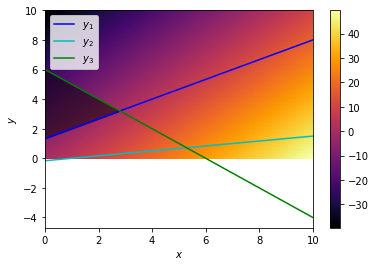
\includegraphics{p8_1_1}
\par\end{center}

\bigskip{}


As we can see from the plot, the objective function is highest at
the rightmost vertex, which is precisely the $x$ and $y$ values
such that 
\begin{eqnarray*}
y=y_{1} & = & y_{3}\\
\frac{2x+4}{3} & = & 6-x\\
2x+4 & = & 18-3x\\
5x & = & 14\\
x & = & \frac{14}{5}\implies y=6-\frac{14}{5}=\frac{16}{5}.
\end{eqnarray*}
$\qed$

\bigskip{}


\bigskip{}


\begin{minipage}[t]{1\columnwidth}%
\begin{shaded}%
\textsf{\textbf{\textcolor{blue}{\large{}Exercise 8.2.}}}{\large \par}

\medskip{}


For each of the following, draw the feasible polygon, identify all
the vertices, and use the Fundamental Theorem to solve the linear
optimization problem (that is, check all the vertices). Give both
the optimal point (optimizer) and the optimum value of the objective
function.
\begin{lyxlist}{00.00.0000}
\item [{$\l i$}] 
\[
\optfour{3x_{1}+x_{2}}{x_{2}+3x_{2}\leq15}{2x_{1}+3x_{2}\leq18}{x_{1}-x_{2}\le4}{x_{1},x_{2}\geq0.}
\]

\item [{$\l{ii}$}] 
\[
\optfour{4x+6y}{-x+y\leq11}{x+y\leq27}{2x+5y\leq90}{x,y\geq0.}
\]
\end{lyxlist}
\end{shaded}%
\end{minipage}\bigskip{}


\textsf{\textbf{\textcolor{black}{\large{}Solution. }}}{\large \par}
\begin{lyxlist}{00.00.0000}
\item [{$\l i$}] \begin{lstlisting}
def p8_2_1(): 
	x = np.linspace(0,10,100) 
	y_1 = 15-x 
	y_2 = (18-2*x)/3 
	y_3 = x-4
	plt.plot(x,y_1,label="$y_1$",c="b")
	plt.plot(x,y_2,label="$y_2$",c="c")
	plt.plot(x,y_3,label="$y_3$",c="g")
	X,Y = np.meshgrid(x,x)
	Z = 3*X + Y 
	plt.pcolormesh(X,Y,Z,cmap="inferno") 
	y_top = np.minimum(y_1,y_2) 
	y_bot = np.maximum(y_3,0) 
	plt.fill_between(x,y_top,y_bot,where=y_top>=y_bot,color="k",alpha=.5) 
	plt.ylabel("$y$") 
	plt.xlabel("$x$") 
	plt.colorbar() 
	plt.legend()
	plt.show()

p8_2_1()
\end{lstlisting}
\end{lyxlist}
\bigskip{}


\begin{center}
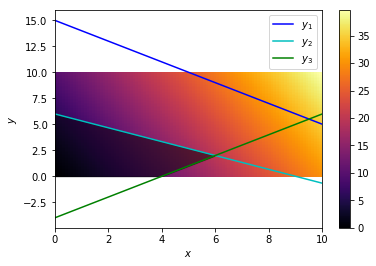
\includegraphics{p8_2_1}
\par\end{center}

\bigskip{}


As we can see, the objective function increases in the northeast direction,
so the vertex at the intersection of $y_{2}$ and $y_{3}$ is where
the optimum is. This is precisely
\begin{eqnarray*}
y=y_{2} & = & y_{3}\\
\frac{18-2x}{3} & = & x-4\\
18-2x & = & 3x-12\\
30 & = & 5x\\
6 & = & x\implies y=6-4=2.
\end{eqnarray*}
$\qed$
\begin{lyxlist}{00.00.0000}
\item [{$\l{ii}$}] \begin{lstlisting}
def p8_2_2(): 
	x = np.linspace(0,20,100) 
	y_1 = 11+x 
	y_2 = 27-x 
	y_3 = (90-2*x)/5
	plt.plot(x,y_1,label="$y_1$",c="b")
	plt.plot(x,y_2,label="$y_2$",c="c")
	plt.plot(x,y_3,label="$y_3$",c="g")
	X,Y = np.meshgrid(x,x) 
	Z = 4*X + 6*Y
	plt.pcolormesh(X,Y,Z,cmap="inferno")
	y_top = 	np.amin(np.array([y_1,y_2,y_3]),axis=0)
	y_bot = 0
	plt.fill_between(x,y_top,y_bot,where=y_top>=y_bot,color="k",alpha=.5)
	plt.ylabel("$y$")
	plt.xlabel("$x$") 
	plt.colorbar() 
	plt.legend() 
	plt.show()

p8_2_2()
\end{lstlisting}
\end{lyxlist}
\bigskip{}


\begin{center}
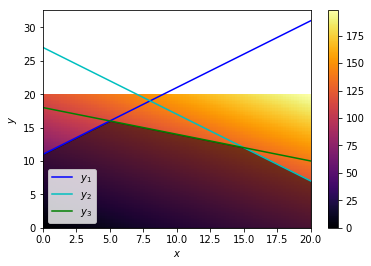
\includegraphics{p8_2_2}
\par\end{center}

\bigskip{}


As we can see above, the optimum is at the vertex of the intersection
between $y_{2}$ and $y_{3}$, which is precisely
\begin{eqnarray*}
y=y_{2} & = & y_{3}\\
27-x & = & \frac{90-2x}{5}\\
135-5x & = & 90-2x\\
45 & = & 3x\\
15 & = & x\implies y=27-15=12.
\end{eqnarray*}
$\qed$

\bigskip{}


\bigskip{}


\begin{minipage}[t]{1\columnwidth}%
\begin{shaded}%
\textsf{\textbf{\textcolor{blue}{\large{}Exercise 8.3.}}}{\large \par}

\medskip{}


Kenny's Toy Co. manufactures two types of toys: a GI Barb soldier
and a Joey doll. A GI Barb soldier sells for $\$12$ and uses $\$5$
worth of raw materials. Each soldier that is manufactured increases
Kenny's general overhead costs by $\$3$. A Joey doll sells for $\$10$
and uses $\$3$ worth of raw material. Each Joey doll built increases
Kenny's overhead costs by $\$4$. The manufacture of soldiers and
dolls require two types of labor: modeling and finishing. A soldier
requires $15$ minutes of finishing labor and $2$ minutes of molding
labor. A Joey doll requires $10$ minutes of finishing and $2$ minutes
of modeling labor. Each week, Kenny can obtain all of the needed raw
material but only $30$ finishing hours and $5$ molding hours of
labor. Demand for GI Barb is unlimited but at most $200$ Joey dolls
are bought each week. Formulate a linear optimization problem in standard
form whose solution would maximize Kenny's profit on these toys.\end{shaded}%
\end{minipage}\bigskip{}


\textsf{\textbf{\textcolor{black}{\large{}Solution. }}}For quantity
vector $\x=\begin{pmatrix}x_{\mathrm{GI\ Barb}}\\
x_{\mathrm{Joey}}
\end{pmatrix}$, we have the problem\textsf{\textbf{\textcolor{black}{\large{} }}}
\[
\optfour{4x_{\mathrm{GI\ Barb}}+3x_{\mathrm{Joey}}}{15x_{\mathrm{GI\ Barb}}+10x_{\mathrm{Joey}}\leq1800}{2x_{\mathrm{GI\ Barb}}+2x_{\mathrm{Joey}}\leq300}{x_{\mathrm{Joey}}\leq200}{\x\succeq\o.}
\]
$\qed$\bigskip{}


\bigskip{}


\begin{minipage}[t]{1\columnwidth}%
\begin{shaded}%
\textsf{\textbf{\textcolor{blue}{\large{}Exercise 8.4.}}}{\large \par}

\medskip{}


Consider the following network, where the weights of each edge represent
the carrying cost per unit of that edge.
\[
\begin{array}{ccccc}
\mycirc{A} & \overset{2}{\rightarrow} & \mycirc{B} & \overset{5}{\rightarrow} & \mycirc{C}\\
\downarrow^{_{5}} & ^{2}\swarrow & ^{_{7}}\downarrow & \searrow^{9} & ^{_{2}}\downarrow\\
\mycirc{D} & \underset{4}{\rightarrow} & \mycirc{E} & \underset{3}{\rightarrow} & \mycirc{F}
\end{array}
\]
Assume that the supply or demand at the nodes is $b_{A}=10$, $b_{B}=1$,
$b_{C}=-2$, $b_{D}=-3$, $b_{E}=4$, $b_{F}=-10$, and that the capacity
of each edge is bounded by $6$. Write a linear optimization problem
in standard form whose solution ives the optimal (cheapest) flow in
this network with these constraints.\end{shaded}%
\end{minipage}\bigskip{}


\textsf{\textbf{\textcolor{black}{\large{}Solution. }}}For flow vector
$\x=\begin{pmatrix}x_{\mathrm{AB}}\\
x_{\mathrm{BC}}\\
\vdots\\
x_{\mathrm{EF}}
\end{pmatrix}$, our problem is
\[
\begin{array}{rl}
\mbox{maximize} & 2x_{\mathrm{AB}}+5x_{\mathrm{AD}}+5x_{\mathrm{BC}}+2x_{\mathrm{BD}}+7x_{\mathrm{BE}}+9x_{\mathrm{BF}}+2x_{\mathrm{CF}}+4x_{\mathrm{DE}}+3x_{\mathrm{EF}}\\
\mbox{subject to} & x_{\mathrm{AB}}+x_{\mathrm{AD}}=10\\
 & x_{\mathrm{BC}}+x_{\mathrm{BD}}+x_{\mathrm{BE}}+x_{\mathrm{BF}}-x_{\mathrm{AB}}=1\\
 & x_{\mathrm{CF}}-x_{\mathrm{BC}}=-2\\
 & x_{\mathrm{DE}}-x_{\mathrm{AD}}-x_{\mathrm{BD}}=-3\\
 & x_{\mathrm{EF}}-x_{\mathrm{BE}}-x_{\mathrm{DE}}=4\\
 & -x_{\mathrm{BF}}-x_{\mathrm{CF}}-x_{\mathrm{EF}}=-10\\
 & \o\preceq\x\preceq\mathbf{6}.
\end{array}
\]
$\qed$\bigskip{}


\bigskip{}


\begin{minipage}[t]{1\columnwidth}%
\begin{shaded}%
\textsf{\textbf{\textcolor{blue}{\large{}Exercise 8.5.}}}{\large \par}

\medskip{}


For each of the linear problems in Exercise 8.2, solve the linear
problem using the simplex algorithm. Show the dictionary after each
pivot. Give both the optimal point (optimizer) and the optimum value
of the objective function. Verify that your answers agree with those
you got in Exercise 8.2.\end{shaded}%
\end{minipage}\bigskip{}


\textsf{\textbf{\textcolor{black}{\large{}Solution. }}}{\large \par}
\begin{lyxlist}{00.00.0000}
\item [{$\l i$}] 
\[
\optfour{3x_{1}+x_{2}}{x_{1}+3x_{2}+w_{1}=15}{2x_{1}+3x_{2}+w_{2}=18}{x_{1}-x_{2}+w_{3}=4}{x_{1},x_{2},w_{1},w_{2},w_{3}\geq0.}
\]
\[
\begin{array}{ccccccc}
\zeta & = &  &  & 3x_{1} & + & x_{2}\\
\hline w_{1} & = & 15 & - & x_{1} & - & 3x_{2}\\
w_{2} & = & 18 & - & 2x_{1} & - & 3x_{2}\\
w_{3} & = & 4 & - & x_{1} & + & x_{2}
\end{array}
\]
\[
\Downarrow
\]
\[
\begin{array}{ccccccc}
\zeta & = & 12 & + & 4x_{2} & - & 3w_{3}\\
\hline w_{1} & = & 11 & - & 4x_{2} & + & w_{3}\\
w_{2} & = & 10 & - & 5x_{2} & + & 2w_{3}\\
x_{1} & = & 4 & + & x_{2} & - & w_{3}
\end{array}
\]
\[
\Downarrow
\]
\[
\begin{array}{ccccccc}
\zeta & = & 20 & - & \frac{4}{5}w_{2} & - & \frac{7}{5}w_{3}\\
\hline w_{1} & = & 3 & + & \frac{4}{5}w_{2} & - & \frac{3}{5}w_{3}\\
x_{2} & = & 2 & - & \frac{1}{5}w_{2} & + & \frac{2}{5}w_{3}\\
x_{1} & = & 6 & - & \frac{1}{5}w_{2} & - & \frac{3}{5}w_{3}.
\end{array}
\]
This problem has optimizer $\begin{pmatrix}6\\
2
\end{pmatrix}$ with optimum $20$.
\item [{$\l{ii}$}] 
\[
\optfour{4x+6y}{-x+3y+w_{1}=11}{x+y+w_{2}=27}{2x+5y+w_{3}=90}{x,y,w_{1},w_{2},w_{3}\geq0.}
\]
\[
\begin{array}{ccccccc}
\zeta & = &  &  & 4x & + & 6y\\
\hline w_{1} & = & 11 & + & x & - & y\\
w_{2} & = & 27 & - & x & - & y\\
w_{3} & = & 90 & - & 2x & - & 5y
\end{array}
\]
\[
\Downarrow
\]
\[
\begin{array}{ccccccc}
\zeta & = & 66 & + & 10x & - & 6w_{1}\\
\hline y & = & 11 & + & x & - & w_{1}\\
w_{2} & = & 16 & - & 2x & + & w_{1}\\
w_{3} & = & 35 & - & 7x & + & 5w_{1}
\end{array}
\]
\[
\Downarrow
\]
\[
\begin{array}{ccccccc}
\zeta & = & 116 & + & \frac{8}{7}w_{1} & - & \frac{10}{7}w_{3}\\
\hline y & = & 16 & - & \frac{2}{7}w_{1} & - & \frac{1}{7}w_{3}\\
w_{2} & = & 6 & - & \frac{3}{7}w_{1} & + & \frac{2}{7}w_{3}\\
x & = & 5 & + & \frac{5}{7}w_{1} & - & \frac{1}{7}w_{3}
\end{array}
\]
\[
\Downarrow
\]
\[
\begin{array}{ccccccc}
\zeta & = & 132 & - & \frac{8}{3}w_{2} & - & \frac{2}{7}w_{3}\\
\hline y & = & 12 & + & \frac{2}{3}w_{2} & - & \frac{1}{3}w_{3}\\
w_{1} & = & 14 & - & \frac{7}{3}w_{2} & + & \frac{2}{3}w_{3}\\
x & = & 15 & - & \frac{5}{3}w_{2} & + & \frac{1}{3}w_{3}.
\end{array}
\]
This problem has optimizer $\begin{pmatrix}15\\
12
\end{pmatrix}$ with optimum $132$.
\end{lyxlist}
$\qed$
\begin{lyxlist}{00.00.0000}
\item [{\bigskip{}
}]~
\end{lyxlist}
\bigskip{}


\begin{minipage}[t]{1\columnwidth}%
\begin{shaded}%
\textsf{\textbf{\textcolor{blue}{\large{}Exercise 8.6.}}}{\large \par}

\medskip{}


Solve the Kenny's Toys linear problem of Exercise 8.3 using the simplex
algorithm. Show the dictionary after each pivot. Give both the optimal
choice of how much of each toy to manufacture and the maximal profit.\end{shaded}%
\end{minipage}\bigskip{}


\textsf{\textbf{\textcolor{black}{\large{}Solution. }}}
\[
\optfour{x_{\mathrm{GI\ Barb}}+3x_{\mathrm{Joey}}}{15x_{\mathrm{GI\ Barb}}+10x_{\mathrm{Joey}}+w_{1}=1800}{2x_{\mathrm{GI\ Barb}}+2x_{\mathrm{Joey}}+w_{2}=300}{x_{\mathrm{Joey}}+w_{3}=200}{\x,\mathbf{w}\succeq\o.}
\]
\[
\begin{array}{ccccccc}
\zeta & = &  &  & 4x_{\mathrm{GI\ Barb}} & + & 3x_{\mathrm{Joey}}\\
\hline w_{1} & = & 1800 & - & 15x_{\mathrm{GI\ Barb}} & - & 10x_{\mathrm{Joey}}\\
w_{2} & = & 300 & - & 2x_{\mathrm{GI\ Barb}} & - & 2x_{\mathrm{Joey}}\\
w_{3} & = & 200 & - & x_{\mathrm{Joey}}
\end{array}
\]
\[
\Downarrow
\]
\[
\begin{array}{ccccccc}
\zeta & = & 450 & + & x_{\mathrm{GI\ Barb}} & - & \frac{3}{2}w_{2}\\
\hline w_{1} & = & 300 & - & 5x_{\mathrm{GI\ Barb}} & + & 5w_{2}\\
x_{\mathrm{Joey}} & = & 150 & - & x_{\mathrm{GI\ Barb}} & - & \frac{1}{2}w_{2}\\
w_{3} & = & 50 & + & x_{\mathrm{GI\ Barb}} & + & \frac{1}{2}w_{2}
\end{array}
\]
\[
\Downarrow
\]
\[
\begin{array}{ccccccc}
\zeta & = & 510 & - & \frac{1}{5}w_{1} & - & \frac{1}{2}w_{2}\\
\hline x_{\mathrm{GI\ Barb}} & = & 60 & - & \frac{1}{5}w_{1} & + & w_{2}\\
x_{\mathrm{Joey}} & = & 90 & + & \frac{1}{5}w_{1} & - & \frac{3}{2}w_{2}\\
w_{3} & = & 110 & - & \frac{1}{5}w_{1} & + & \frac{3}{2}w_{2}.
\end{array}
\]
This problem has optimizer $\x=\begin{pmatrix}x_{\mathrm{GI\ Barb}}\\
x_{\mathrm{Joey}}
\end{pmatrix}=\begin{pmatrix}60\\
90
\end{pmatrix}$ with optimum \textbf{$\$150$}.$\qed$\bigskip{}


\bigskip{}


\begin{minipage}[t]{1\columnwidth}%
\begin{shaded}%
\textsf{\textbf{\textcolor{blue}{\large{}Exercise 8.7.}}}{\large \par}

\medskip{}


Solve the following linear problems using the simplex algorithm. Show
the dictionary after each pivot. If there is a solution, give an optimal
point and the optimal value. If there isn't a solution, tell whether
the problem is unbounded or infeasible.
\begin{lyxlist}{00.00.0000}
\item [{$\l i$}] 
\[
\optfour{x_{1}+2x_{2}}{-4x_{1}-2x_{2}\leq-8}{-2x_{1}+3x_{2}\leq6}{x_{1}\leq3}{x_{1},x_{2}\geq0.}
\]

\item [{$\l{ii}$}] 
\[
\optfour{5x_{1}+2x_{2}}{5x_{1}+3x_{2}\leq15}{3x_{1}+5x_{2}\leq15}{4x_{1}-3x_{2}\leq-12}{x_{1},x_{2}\geq0.}
\]

\item [{$\l{iii}$}] 
\[
\optthree{-3x_{1}+x_{2}}{x_{2}\leq4}{-2x_{1}+3x_{2}\leq6}{x_{1},x_{2}\geq0.}
\]
\end{lyxlist}
\end{shaded}%
\end{minipage}\bigskip{}


\textsf{\textbf{\textcolor{black}{\large{}Solution. }}}{\large \par}
\begin{lyxlist}{00.00.0000}
\item [{$\l i$}] We have
\[
\optfour{x_{1}+2x_{2}}{-4x_{1}-2x_{2}+x_{3}-8}{-2x_{1}+3x_{2}+x_{4}=6}{x_{1}+x_{5}=3}{x_{1},x_{2},x_{3},x_{4},x_{5}\geq0,}
\]
with auxiliary problem
\[
\optfour{-x_{0}}{-4x_{1}-2x_{2}+x_{3}-x_{0}=-8}{-2x_{1}+3x_{2}+x_{4}-x_{0}=6}{x_{1}+x_{5}-x_{0}=3}{x_{0},x_{1},x_{2},x_{3},x_{4},x_{5}\geq0.}
\]
Solving using simplex, we have:
\[
\begin{array}{ccccccccc}
\zeta & = &  &  &  &  &  & - & x_{0}\\
\hline x_{3} & = & -8 & + & 4x_{1} & + & 2x_{2} & + & x_{0}\\
x_{4} & = & 6 & + & 2x_{1} & - & 3x_{2} & + & x_{0}\\
x_{5} & = & 3 & - & x_{1} &  &  & + & x_{0}
\end{array}
\]
\[
\Downarrow
\]
\[
\begin{array}{ccccccccc}
\zeta & = & -8 & + & 4x_{1} & + & 2x_{3} & - & x_{3}\\
\hline x_{0} & = & 8 & - & 4x_{1} & - & 2x_{2} & + & x_{3}\\
x_{4} & = & 14 & - & 2x_{1} & - & 5x_{2} & + & x_{3}\\
x_{5} & = & 11 & - & 5x_{1} & - & 2x_{2} & + & x_{3}
\end{array}
\]
\[
\Downarrow
\]
\[
\begin{array}{ccccccccc}
\zeta & = &  &  &  &  &  & - & x_{0}\\
\hline x_{1} & = & 2 & - & \frac{1}{2}x_{2} & + & \frac{1}{4}x_{3} & - & \frac{1}{4}x_{0}\\
x_{4} & = & 10 & - & 4x_{2} & + & \frac{1}{2}x_{3} & + & \frac{1}{2}x_{0}\\
x_{5} & = & 1 & + & \frac{1}{2}x_{2} & - & \frac{1}{4}x_{3} & + & \frac{5}{4}x_{0}
\end{array}
\]
\[
\Downarrow
\]
\[
\begin{array}{ccccccccc}
\zeta & = & 2 & + & \frac{3}{2}x_{2} & + & \frac{1}{4}x_{3}\\
\hline x_{1} & = & 2 & - & \frac{1}{2}x_{2} & + & \frac{1}{4}x_{3}\\
x_{4} & = & 10 & - & 4x_{2} & + & \frac{1}{2}x_{3}\\
x_{5} & = & 1 & + & \frac{1}{2}x_{2} & - & \frac{1}{4}x_{3}
\end{array}
\]
\[
\Downarrow
\]
\[
\begin{array}{ccccccccc}
\zeta & = & 3 & + & 2x_{2} & - & x_{5}\\
\hline x_{1} & = & 3 &  &  & - & x_{5}\\
x_{4} & = & 12 & - & 3x_{2} & - & 2x_{5}\\
x_{3} & = & 4 & + & 2x_{2} & - & 4x_{5}
\end{array}
\]
\[
\Downarrow
\]
\[
\begin{array}{ccccccccc}
\zeta & = & 11 & - & \frac{2}{3}x_{4} & - & \frac{7}{3}x_{5}\\
\hline x_{1} & = & 3 &  &  & - & x_{5}\\
x_{2} & = & 4 & - & \frac{1}{3}x_{4} & - & \frac{2}{3}x_{5}\\
x_{3} & = & 4 & - & \frac{2}{3}x_{4} & - & \frac{16}{3}x_{5}.
\end{array}
\]
This problem has optimizer $\begin{pmatrix}x_{1}\\
x_{2}
\end{pmatrix}=\begin{pmatrix}3\\
4
\end{pmatrix}$ and optimum $11$.
\item [{$\l{ii}$}] We have
\[
\optfour{5x_{1}+2x_{2}}{5x_{1}+3x_{2}+x_{3}=15}{3x_{1}+5x_{2}+x_{4}=15}{4x_{1}-3x_{2}+x_{4}=-12}{x_{1},x_{2},x_{3},x_{4},x_{5}\geq0,}
\]
 with auxiliary problem
\[
\optfour{-x_{0}}{5x_{1}+3x_{2}+x_{3}-x_{0}=15}{3x_{1}+5x_{2}+x_{4}-x_{0}=15}{4x_{1}-3x_{2}+x_{5}-x_{0}=-12}{x_{0},x_{1},x_{2},x_{3},x_{4},x_{5}\geq0.}
\]
Using simplex, we have:
\[
\begin{array}{ccccccccc}
\zeta & = &  &  &  &  &  & - & x_{0}\\
\hline x_{3} & = & 15 & - & 5x_{1} & - & 3x_{2} & + & x_{0}\\
x_{4} & = & 15 & - & 3x_{1} & - & 5x_{2} & + & x_{0}\\
x_{5} & = & -12 & - & 4x_{1} & + & 3x_{2} & + & x_{0}
\end{array}
\]
\[
\Downarrow
\]
\[
\begin{array}{ccccccccc}
\zeta & = & -12 & - & 4x_{1} & + & 3x_{2} & - & x_{5}\\
\hline x_{3} & = & 27 & - & x_{1} & - & 6x_{2} & + & x_{5}\\
x_{4} & = & 27 & + & x_{1} & - & 8x_{2} & + & x_{5}\\
x_{0} & = & 12 & + & 4x_{1} & - & 3x_{2} & + & x_{5}
\end{array}
\]
\[
\Downarrow
\]
\[
\begin{array}{ccccccccc}
\zeta & = & -\frac{15}{8} & - & \frac{29}{8}x_{1} & - & \frac{3}{8}x_{4} & - & \frac{5}{8}x_{5}\\
\hline x_{3} & = & \frac{27}{4} & - & \frac{7}{4}x & + & \frac{3}{4}x_{4} & + & \frac{1}{4}x_{5}\\
x_{2} & = & \frac{27}{8} & + & \frac{1}{8}x_{1} & - & \frac{1}{8}x_{4} & + & \frac{1}{8}x_{5}\\
x_{0} & = & \frac{15}{8} & + & \frac{29}{8}x_{1} & + & \frac{3}{8}x_{4} & + & \frac{5}{8}x_{5}.
\end{array}
\]
Unfortunately, there are no feasible solutions.
\item [{$\l{iii}$}] We have
\[
\optthree{-3x_{1}+x_{2}}{x_{2}+x_{3}=4}{-2x_{1}+3x_{2}+x_{4}=6}{x_{1},x_{2},x_{3},x_{4}\geq0.}
\]
 Solving using simplex, we have:
\[
\begin{array}{ccccccc}
\zeta & = &  & - & 3x_{1} & + & x_{2}\\
\hline x_{3} & = & 4 &  &  & - & x_{2}\\
x_{4} & = & 6 & + & 2x_{1} & - & 3x_{2}
\end{array}
\]
\[
\Downarrow
\]
\[
\begin{array}{ccccccc}
\zeta & = & 2 & - & \frac{7}{3}x_{1} & - & \frac{1}{3}x_{4}\\
\hline x_{3} & = & 2 & - & \frac{2}{3}x_{1} & + & \frac{1}{3}x_{4}\\
x_{2} & = & 2 & + & \frac{2}{3}x_{1} & - & \frac{1}{3}x_{4}.
\end{array}
\]
This problem has optimizer $\begin{pmatrix}0\\
2
\end{pmatrix}$ with optimum $2$.
\end{lyxlist}
$\qed$
\begin{lyxlist}{00.00.0000}
\item [{\bigskip{}
}]~
\end{lyxlist}
\bigskip{}


\begin{minipage}[t]{1\columnwidth}%
\begin{shaded}%
\textsf{\textbf{\textcolor{blue}{\large{}Exercise 8.8.}}}{\large \par}

\medskip{}


Give an example of a three-dimensional linear problem where the feasible
region is closed and unbounded, but where the objective function still
has a unique feasible maximizer.\end{shaded}%
\end{minipage}\bigskip{}


\textsf{\textbf{\textcolor{black}{\large{}Solution. }}}
\[
\optfive{-x_{1}-x_{2}-x_{3}}{-x_{1}+x_{2}\leq1}{x_{1}-x_{2}\leq1}{x_{1}-x_{3}\leq1}{-x_{1}+x_{3}\leq1}{\x\succeq\o.}
\]
$\qed$\bigskip{}


\bigskip{}


\begin{minipage}[t]{1\columnwidth}%
\begin{shaded}%
\textsf{\textbf{\textcolor{blue}{\large{}Exercise 8.9.}}}{\large \par}

\medskip{}


Give an example of a three-dimensional linear problem where the feasible
region is closed and unbounded and where the objective function has
no maximizer.\end{shaded}%
\end{minipage}\bigskip{}


\textsf{\textbf{\textcolor{black}{\large{}Solution. }}}
\[
\optfive{x_{1}+x_{2}+x_{3}}{-x_{1}+x_{2}\leq1}{x_{1}-x_{2}\leq1}{x_{1}-x_{3}\leq1}{-x_{1}+x_{3}\leq1}{\x\succeq\o.}
\]
$\qed$\bigskip{}


\bigskip{}


\begin{minipage}[t]{1\columnwidth}%
\begin{shaded}%
\textsf{\textbf{\textcolor{blue}{\large{}Exercise 8.10.}}}{\large \par}

\medskip{}


Give an example of a three-dimensional linear problem where the feasible
region is empty.\end{shaded}%
\end{minipage}\bigskip{}


\textsf{\textbf{\textcolor{black}{\large{}Solution. }}}
\[
\optfive{x_{1}+x_{2}+x_{3}}{-x_{1}+x_{2}\leq-1}{x_{1}-x_{2}\leq-1}{x_{1}-x_{3}\leq-1}{-x_{1}+x_{3}\leq-1}{\x\succeq\o.}
\]
$\qed$\bigskip{}


\bigskip{}


\begin{minipage}[t]{1\columnwidth}%
\begin{shaded}%
\textsf{\textbf{\textcolor{blue}{\large{}Exercise 8.11.}}}{\large \par}

\medskip{}


Give an example of a three-dimensional linear problem where the feasible
region is nonempty, closed, and bounded, but $\o$ is not feasible.
Write an auxiliary problem (for which $\o$ is feasible) whose solution
gives a feasible vertex for starting the original problem.\end{shaded}%
\end{minipage}\bigskip{}


\textsf{\textbf{\textcolor{black}{\large{}Solution. }}}
\[
\begin{array}{rl}
\mbox{maximize} & x_{1}+x_{2}+x_{3}\\
\mbox{subject to} & -x_{1}+x_{2}\leq1\\
 & x-x_{2}\leq1\\
 & x_{1}-x_{3}\leq1\\
 & -x_{1}+x_{3}\leq1\\
 & -x_{1}-x_{2}-x_{3}\leq-1\\
 & x_{1}+x_{2}+x_{3}\leq5\\
 & \x\succeq\o,
\end{array}
\]
with corresponding auxiliary problem
\[
\begin{array}{rl}
\mbox{maximize} & -x_{0}\\
\mbox{subject to} & -x_{1}+x_{2}+x_{0}\leq1\\
 & x_{1}-x_{2}+x_{0}\leq1\\
 & x_{1}-x_{3}+x_{0}\leq1\\
 & -x+x_{3}+x_{0}\leq1\\
 & -x_{1}-x_{2}-x_{3}+x_{0}\leq-1\\
 & x_{1}+x_{2}+x_{3}+x_{0}\leq5\\
 & \x\succeq\o.
\end{array}
\]
$\qed$\bigskip{}


\bigskip{}


\begin{minipage}[t]{1\columnwidth}%
\begin{shaded}%
\textsf{\textbf{\textcolor{blue}{\large{}Exercise 8.12.}}}{\large \par}

\medskip{}


Solve the following linear problem using Bland's rule to resolve degeneracy.
Show the dictionary after each pivot. Give the optimal point and the
optimum value of the objective function.
\[
\optfour{10x_{1}-57x_{2}-9x_{3}-24x_{4}}{0.5x_{1}-1.5x_{2}-0.5x_{3}+x_{4}\leq0}{0.5x_{1}-5.5x_{2}-2.5x_{3}+9x_{4}\leq0}{x_{1}\leq1}{x_{1},x_{2},x_{3},x_{4}\geq0.}
\]
\end{shaded}%
\end{minipage}\bigskip{}


\textsf{\textbf{\textcolor{black}{\large{}Solution. }}}We have
\[
\optfour{10x_{1}-57x_{2}-9x_{3}-24x_{4}}{0.5x_{1}-1.5x_{2}-0.5x_{3}+x_{4}+x_{5}=0}{0.5x_{1}-5.5x_{2}-2.5x_{3}+9x_{4}+x_{6}=0}{x_{1}+x_{7}=0}{x_{1},x_{2},x_{3},x_{4},x_{5},x_{6},x_{7}\geq0.}
\]
Solving using simplex, we have
\[
\begin{array}{ccccccccccc}
\zeta & = &  &  & 10x_{1} & - & 57x_{2} & - & 9x_{3} & - & 24x_{4}\\
\hline x_{5} & = &  & - & 0.5x_{1} & + & 1.5x_{2} & + & 0.5x_{3} & - & x_{4}\\
x_{6} & = &  & - & 0.5x_{1} & + & 5.5x_{2} & + & 2.5x_{3} & - & 9x_{4}\\
x_{7} & = & 1 & - & x_{1}
\end{array}
\]
\[
\Downarrow
\]
\[
\begin{array}{ccccccccccc}
\zeta & = &  & - & 27x_{2} & + & x_{3} & - & 44x_{4} & - & 20x_{5}\\
\hline x_{1} & = &  &  & 3x_{2} & + & x_{3} & - & 2x_{4} & - & 2x_{5}\\
x_{6} & = &  &  & 4x_{2} & + & 2x_{3} & - & 8x_{4} & + & x_{5}\\
x_{7} & = & 1 & - & 3x_{2} & - & x_{3} & + & 2x_{4} & + & 2x_{5}
\end{array}
\]
\[
\Downarrow
\]
\[
\begin{array}{ccccccccccc}
\zeta & = & 1 & - & 30x_{2} & - & 42x_{4} & - & 18x_{5} & - & x_{7}\\
\hline x_{1} & = & 1 &  &  &  &  &  &  & - & x_{7}\\
x_{6} & = & 2 & - & 2x_{2} & - & 4x_{4} & + & 5x_{5} & - & 2x_{7}\\
x_{3} & = & 1 & - & 3x_{2} & + & 2x_{4} & + & 2x_{5} & - & x_{7}.
\end{array}
\]
Our optimizer is $\begin{pmatrix}x_{1}\\
x_{2}\\
x_{3}\\
x_{4}
\end{pmatrix}=\begin{pmatrix}1\\
0\\
1\\
0
\end{pmatrix}$ with optimum $1$.$\qed$\bigskip{}


\bigskip{}


\begin{minipage}[t]{1\columnwidth}%
\begin{shaded}%
\textsf{\textbf{\textcolor{blue}{\large{}Exercise 8.15.}}}{\large \par}

\medskip{}


Prove the Weak Duality Theorem: If $\x$ is a primal feasible point
and $\y$ is any feasible point of the dual then $\mathbf{c}\t\x\leq\b\t\y$.\end{shaded}%
\end{minipage}\bigskip{}


\textsf{\textbf{\textcolor{black}{\large{}Solution. }}}Let $\x\in\r^{n}$
be feasible for the primal and $\y\in\R^{m}$ be feasible for the
dual. It follows that $\A\x\leq\b$ and $\A\t\y\leq\mathbf{c}$, for
which it then follows
\begin{eqnarray*}
\b & \geq & \A\x\\
 & \Downarrow\\
\b\t & \geq & \x\t\A\t\\
 & \Downarrow\\
\b\t\y & \geq & \x\t\A\t\y\\
 & \geq & \x\t\mathbf{c}\\
 & \geq & \mathbf{c}\t\x.
\end{eqnarray*}
$\qed$\bigskip{}


\bigskip{}


\begin{minipage}[t]{1\columnwidth}%
\begin{shaded}%
\textsf{\textbf{\textcolor{blue}{\large{}Exercise 8.17.}}}{\large \par}

\medskip{}


Prove that the dual of the dual of a linear problem is the primal
problem.\end{shaded}%
\end{minipage}\bigskip{}


\textsf{\textbf{\textcolor{black}{\large{}Solution. }}}For the primal
problem
\[
\opttwo{\mathbf{c}\t\x}{\A\x\preceq\b}{\x\succeq\o}
\]
with dual
\[
\opttwo{\b\t\y}{\A\t\y\succeq\mathbf{c}}{\y\succeq\o,}
\]
yielding double dual
\[
\opttwo{\mathbf{c}\t\z}{\left(\A\t\right)\t\z\succeq\b}{\z\succeq\o,}
\]
which is simply
\[
\opttwo{\mathbf{c}\t\z}{\A\z\succeq\b}{\z\succeq\o.}
\]
$\qed$\bigskip{}


\bigskip{}


\begin{minipage}[t]{1\columnwidth}%
\begin{shaded}%
\textsf{\textbf{\textcolor{blue}{\large{}Exercise 8.18.}}}{\large \par}

\medskip{}


Give the dual of the linear problem
\[
\optfour{x_{1}+x_{2}}{2x_{1}+x_{2}\leq3}{x_{1}+3x_{2}\leq5}{2x_{1}+3x_{2}\leq4}{x_{1},x_{2}\geq0.}
\]
\end{shaded}%
\end{minipage}\bigskip{}


\textsf{\textbf{\textcolor{black}{\large{}Solution. }}}Our primal
problem is
\[
\optfour{x_{1}+x_{2}}{2x_{1}+x_{2}+w_{1}=3}{x_{1}+3x_{2}+w_{2}=5}{2x_{1}+3x_{2}+w_{3}=4}{x_{1},x_{2},w_{1},w_{2},w_{3}\geq0.}
\]
Solving with simplex, we have
\[
\begin{array}{ccccccc}
\zeta & = &  &  & x_{1} & + & x_{2}\\
\hline w_{1} & = & 3 & - & 2x_{1} & - & x_{2}\\
x_{2} & = & 5 & - & x_{1} & - & 3x_{2}\\
x_{5} & = & 4 & - & 2x_{1} & - & 3x_{2}
\end{array}
\]
\[
\Downarrow
\]
\[
\begin{array}{ccccccc}
\zeta & = & \frac{3}{2} & + & \frac{1}{2}x_{2} & - & \frac{1}{2}w_{1}\\
\hline x_{1} & = & \frac{3}{2} & - & \frac{1}{2}x_{2} & - & \frac{1}{2}w_{1}\\
w_{2} & = & \frac{7}{2} & - & \frac{5}{2}x_{2} & + & \frac{1}{2}w_{1}\\
w_{3} & = & 1 & - & 2x_{2} & + & w_{1}
\end{array}
\]
\[
\Downarrow
\]
\[
\begin{array}{ccccccc}
\zeta & = & \frac{7}{4} & - & \frac{1}{4}w_{1} & - & \frac{1}{4}w_{1}\\
\hline x_{1} & = & \frac{5}{4} & - & \frac{3}{4}w_{1} & + & \frac{1}{4}w_{3}\\
w_{2} & = & \frac{9}{4} & - & \frac{3}{4}w_{1} & + & \frac{5}{4}w_{3}\\
x_{2} & = & \frac{1}{2} & + & \frac{1}{2}w_{1} & - & \frac{1}{2}w_{3}.
\end{array}
\]
with optimizer $\begin{pmatrix}\frac{5}{4}\\
\frac{1}{2}
\end{pmatrix}$ and optimum $\frac{7}{4}$. The dual problem is
\[
\optthree{-3y_{1}-5y_{2}-4y_{3}}{-2y_{1}-y_{2}-2y_{3}+v_{1}-v_{0}=-1}{-y_{1}-3y_{2}-3y_{3}+v_{2}-v_{0}=-1}{y_{1},y_{2},y_{3},v_{1},v_{2}\geq0.}
\]
Solving through simplex, we have
\[
\begin{array}{ccccccccccc}
\zeta & = &  &  &  &  &  &  &  & - & v_{0}\\
\hline v_{1} & = & -1 & + & 2y_{1} & + & y_{2} & + & 2y_{3} & + & v_{0}\\
v_{2} & = & -1 & + & y_{1} & + & 3y_{2} & + & 3y_{3} & + & v_{0}
\end{array}
\]
\[
\Downarrow
\]
\[
\begin{array}{ccccccccccc}
\zeta & = & -1 & + & 2y_{1} & + & y_{2} & + & 2y_{3} & - & v_{1}\\
\hline v_{0} & = & 1 & - & 2y_{1} & - & y_{2} & - & 2y_{3} & + & v_{1}\\
v_{2} & = &  & - & y_{1} & + & 2y_{2} & + & y_{3} & + & v_{1}
\end{array}
\]
\[
\Downarrow
\]
\[
\begin{array}{ccccccccccc}
\zeta & = &  &  &  &  &  &  &  & - & v_{0}\\
\hline y_{2} & = & 1 & - & 2y_{1} & - & 2y_{3} & + & v_{1} & - & v_{0}\\
v_{2} & = & 2 & - & 5y_{1} & - & 3y_{3} & + & 3v_{1} & - & 2v_{0}
\end{array}
\]
\[
\Downarrow
\]
\[
\begin{array}{ccccccccccc}
\zeta & = & -2 & + & y_{1} & - & 3y_{2} & - & 2v_{1}\\
\hline y_{3} & = & \frac{1}{2} & - & y_{1} & - & \frac{1}{2}y_{2} & + & \frac{1}{2}v_{1}\\
v_{2} & = & \frac{1}{2} & - & 2y_{1} & + & \frac{3}{2}y_{2} & + & \frac{3}{2}v_{1}
\end{array}
\]
\[
\Downarrow
\]
\[
\begin{array}{ccccccccccc}
\zeta & = & -\frac{7}{4} & - & \frac{3}{2}y_{2} & - & \frac{5}{4}v_{1} & - & \frac{1}{2}v_{2}\\
\hline y_{3} & = & \frac{1}{4} & - & \frac{3}{2}y_{2} & - & \frac{1}{4}v_{1} & + & \frac{1}{2}v_{2}\\
y_{1} & = & \frac{1}{4} & + & \frac{3}{2}y_{2} & + & \frac{3}{4}v_{1} & - & \frac{1}{2}v_{2}.
\end{array}
\]
with optimizer $\begin{pmatrix}\frac{1}{4}\\
0\\
\frac{1}{4}
\end{pmatrix}$ and optimum $\frac{7}{4}$.$\qed$
\end{document}
